\documentclass[12pt]{article}

%Technometrics specified margins:

% NOTE: To produce blinded version, replace "0" with "1" below.
\newcommand{\blind}{0}

% DON'T change margins - should be 1 inch all around.
\addtolength{\oddsidemargin}{-.5in}%
\addtolength{\evensidemargin}{-.5in}%
\addtolength{\textwidth}{1in}%
\addtolength{\textheight}{1.3in}%
\addtolength{\topmargin}{-.8in}%
\usepackage{psfrag,epsf,enumerate}

%\usepackage[margin=1.1in]{geometry}
\usepackage{color, amssymb, amsmath,bm,verbatim}
\usepackage{rotating, subfig, setspace, tikz}
\usepackage{graphicx, graphics, epsfig}
\usepackage{multirow,multicol}
\usepackage{natbib}
\newcommand{\tr}{{\mathbf{tr}}}
\newcommand{\rmk}{{\mathcal{K}}}
\newcommand{\I}{{\mathrm{I}}}
\newcommand{\E}{{\mathrm{E}}}
\newcommand{\B}{{\mathcal{B}}}
\newcommand{\bmo}{{\bm{o}}}
\newcommand{\R}{{\mathbb{R}}}
\newcommand{\cov}{{\mathrm{Cov}}}
\newcommand{\Log}{\text{Log}}
\newcommand{\M}{\mathcal{M}}
\newcommand{\refeq}[1]{{eq.~(\ref{#1})}}

\newcommand{\ProjMean}{{\widehat{\bm S}_E}}
\newcommand{\ProjMedian}{{\widetilde{\bm S}_E}}
\newcommand{\GeomMean}{{\widehat{\bm S}_R}}
\newcommand{\GeomMedian}{{\widetilde{\bm S}_R}}
\newcommand{\Rdist}{{d_R}}
\newcommand{\Edist}{{d_E}}

\DeclareMathOperator*{\argmax}{arg\,max}
\DeclareMathOperator*{\argmin}{arg\,min}
\newcommand{\blue}[1]{{\color{blue} #1}}
\newcommand{\red}[1]{{\color{red} #1}}
\newcommand{\green}[1]{{\color{green} #1}}
\newcommand{\hh}[1]{{\color{orange} #1}}

%\pagestyle{plain}
%\bibliographystyle{plainnat}
\bibliographystyle{abbrvnat}
\setcounter{section}{0}
\bibpunct{(}{)}{;}{a}{,}{;}
\graphicspath{{images/}}
%\setlength{\parindent}{0pt}
\begin{document}
\setcounter{table}{4}
\setcounter{figure}{9}
\appendix

\section{Riemannian and Euclidean Distance}
\label{sec:appendix2}
In this section we show that for $\bm R_i\in SO(3)$ for $i=1,2$, $\Edist(\bm R_1,\bm R_2)=2\sqrt{2}\sin[\Rdist(\bm R_1,\bm R_2)/2]$ as stated in Section 5.

\begin{figure}[h!]
\begin{center}
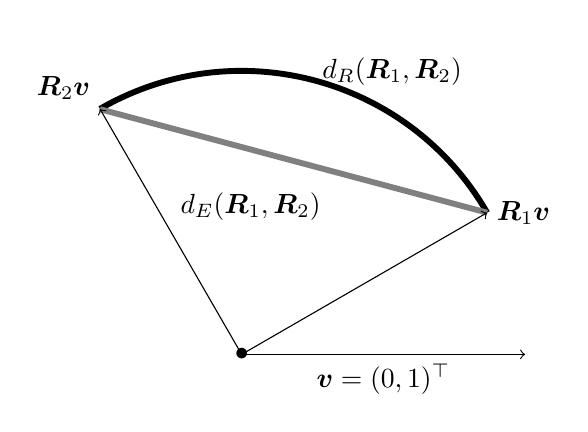
\begin{tikzpicture}[scale=.9]
%\draw (0,0) circle (4cm);
\draw (0,0) node {$\bullet$};
\draw (3.464102,2) node[anchor =  west]{$\bm R_1\bm v$};
\draw [->] (0,0)--(4,0);
%\draw [->] (4,0) arc (0:30:4cm);
\draw (2,0) node[anchor = north]{$\bm v=(0,1)^\top$};
\draw (-2,3.46) node[anchor = south east]{$\bm R_2\bm v$};
\draw [line width=.75mm] (3.464102,2) arc (30:120:4cm);
\draw[line width=.75mm, color=gray] (-2,3.46)--(3.464102,2);
\draw [->](0,0) -- (-2,3.464102);
\draw [->](0,0)--(3.464102,2);
\draw (1,3.66) node[anchor= south west]{$\Rdist (\bm R_1,\bm R_2)$};
\draw (-1,1.75) node[anchor= south west]{$\Edist (\bm R_1,\bm R_2)$};
%\draw (0,0) circle (4cm);
%\draw (0,0) node {$\bullet$};
%\draw (0,0)--(4,0) node[anchor =  west]{$o_1$};
%\draw (4,0) node[anchor =  west]{$\bm R_1$};
%\draw (0,0)--(-2,3.46) node[anchor = south east]{$o_2$};
%\draw (-2,3.46) node[anchor = south east]{$\bm R_2$};
%\draw[line width=.75mm] (4,0) arc (0:120:4cm);
%\draw[line width=.75mm, color=gray] (-2,3.46)--(4,0);
%\draw (0,0)--(2,3.46) node[anchor= south west]{$\alpha$};
%\draw (2,3.46) node[anchor= south west]{$\Rdist (\bm R_1,\bm R_2)$};
%\draw (-1.25,0.73) node[anchor= south west]{$\Edist (\bm R_1,\bm R_2)$};
%\draw (3/8,.7)[->] arc (60:120:.75cm);
%\draw (0,1.2) node {$\frac{\alpha}{2}$};
%\draw (0,2.8) node {$\frac{\beta}{2}$};
%\draw (2,0) node[anchor=north]{1};
\end{tikzpicture}
\end{center}
\vspace{-.25cm}
\caption{An illustration of the Euclidean and Riemannian distance metric on $SO(2)$. To simplify the visualization we use $SO(2)$ in place of $SO(3)$.   $\bm R_1$, $\bm R_2$ are $2\times2$ rotation matrices in $SO(2)$, where $\bm R_1\bm v$ and $\bm R_2\bm v$ are points on the $\mathbb R^2$ unit circle after rotating $\bm v = (0,1)^{\top}$ by  $\bm R_1$ and $\bm R_2$, respectively.  $\Rdist (\bm R_1,\bm R_2)$ is displayed by the curved line (black), $\Edist (\bm R_1,\bm R_2)$ by the straight line (gray).}
\label{fig:dEvsdG2} 
\end{figure}

\noindent In Figure \ref{fig:dEvsdG2} the Riemannian distance between $\bm R_1$ and $\bm R_2\in SO(2)$ is given by $\Rdist(\bm R_1,\bm R_2)$ and is indicated with the thick black arc.  The Euclidean distance is given by $\Edist(\bm R_1,\bm R_2)$ and is indicated by the straight gray line.  Using geometry it is clear that half of the Euclidean distance is the sine of half of the Riemannian distance, i.e.
\[
\Edist(\bm R_1,\bm R_2)=2\sin\left(\frac{\Rdist(\bm R_1,\bm R_2)}{2}\right).
\]

\noindent We claim that this can be extended to $\bm R_1,\bm R_2 \in SO(3)$ as 
\begin{equation}\label{EvR}
\Edist (\bm{R}_1,\bm{R}_2)=2^{3/2}\sin\left(\frac{\Rdist(\bm{R}_1,\bm{R}_2)}{2}\right)
\end{equation}
%\emph{Proof:}\\
for $\bm{R}_1,\bm{R}_2\in SO(3)$.  To show this recall that if $\tr(\bm R_1^\top\bm R_2)=1+2\cos(r)$ then $|r|=\Rdist(\bm R_1,\bm R_2)$.  For the case $|r|=0$, \eqref{EvR} holds trivially so consider the case $|r|>0$.  By definition of $\Edist (\bm R_1,\bm R_2)$:
\begin{align*}
\Edist (\bm R_1,\bm R_2)^2
&=||\bm R_1-\bm R_2||_F^2\\
&=\tr\left[(\bm R_1-\bm R_2)^\top(\bm R_1-\bm R_2)\right]\\
%&=\tr\left[(\bm R_1^\top-\bm R_2^\top)(\bm R_1-\bm R_2)\right]\\
&=\tr\left[\bm R_1^\top\bm R_1+\bm R_2^\top\bm R_2-\bm R_2^\top\bm R_1-\bm R_1^\top\bm R_2\right]\\
&=\tr\left[2\bm{I}-\bm R_2^\top\bm R_1-\bm R_1^\top\bm R_2\right]\\
&=2\tr(\bm{I})-\tr(\bm R_2^\top\bm R_1)-\tr(\bm R_1^\top\bm R_2)\\
&=6-2\tr(\bm R_1^\top\bm R_2)\\
%&=6-2(1+2\cos(r))\\
&=6-2-4\cos(|r|)\\
&=8\left(\frac{1-\cos(|r|)}{2}\right)\\
&=8\sin^2\left(\frac{|r|}{2}\right)\\
&=\left[2^{3/2}\sin\left(\frac{|r|}{2}\right)\right]^2\\
&=\left[2^{3/2}\sin\left(\frac{\Rdist(\bm R_1,\bm R_2)}{2}\right)\right]^2
\end{align*}
Taking square roots on both sides gives \eqref{EvR}.

\section{Sampling Process}
\label{sec:appendix1}
\subsection{Circular-von Mises-based distribution}

To simulate a random sample of rotation angles from the circular-von Mises-based distribution we follow the  algorithm proposed by Best and Fisher (1979).  The algorithm is available in the IMSL Library (1991) and is implemented as follows.  Let $\mu=0$ denote the mean of the target angular distribution and $\kappa$ its concentration parameter.  We define constants $a, b$ and $d$ as
$a\equiv 1+\sqrt{1+4\kappa^2},\quad b\equiv(a-\sqrt{2a}),\quad d\equiv(1+b^2)/2b.$
In steps one, two and four we generate three new observations $u_1$, $u_2$ and $u_3$,  each from a uniform distribution defined over the interval $(0,1)$. 
\begin{enumerate}
\item Set $z=\cos(\pi u_1)$, $f=(1+dz)/(z+d)$ and $c=\kappa(d-f)$.
\item If $c(2-c)-u_2>0$ go to step 4.
\item If $\log(c/u_2)+1-c<0$ return to step 1.
\item Set $r=\text{sign}(u_3-0.5)\cos^{-1}(f)$
\end{enumerate}
It follows that  $r$ is distributed according to the circular-von Mises$(\kappa)$ distribution.

\subsection{Cayley distribution}%\hfill

To simulate rotation angles from a Cayley distribution we make use of a result given in Le{\'o}n et al., (2006). If the angle $r$ follows a Cayley distribution it holds that $\frac{1+\cos r}{2} \sim \text{Beta}(\kappa+1/2, 3/2)$.  Hence, angles following the Cayley distribution can be simulated through composition: 
\begin{enumerate}
\item Generate $Z\sim$Bernoulli(0.5) and set  $Y=1-2Z$
\item Independently generate $X\sim$ Beta$(\kappa+1/2, 3/2)$
\item Set $r= \frac{Y}{2}\cos^{-1}(2X-1)$
\end{enumerate}
Angles $r$ simulated in this fashion follow a Cayley$(\kappa)$ distribution.

\subsection{matrix Fisher distribution}%\hfill

Simulation from the matrix Fisher distribution is achieved through a rejection algorithm.  Let  $\mathrm{C_F}(r|\kappa)$ denote the matrix Fisher density.% as given in Table~\ref{tab:ang.dens}. %and $Y\sim$ Uniform$(-\pi,\pi]$.

\begin{enumerate}
\item Define $M=\frac{1}{2\kappa}e^{2\kappa - 1}\frac{1}{\mathbf{I}_0(2\kappa)-\mathbf{I}_1(2\kappa)}$
\item Generate $U\sim$ Uniform$(0,1)$ and $Y\sim$ Uniform$(-\pi,\pi]$, where $U$ and $Y$ are independent.
\item If $U<\frac{1}{M}\mathrm{C_F}(Y|\kappa)$, accept $Y$; otherwise return to step (2)
\end{enumerate}

%\subsection{Rotation Matrix Formulation}
%
%Given a set of randomly generated angles of rotation $r_1,\ldots, r_n$, the rotation matrix formulation following from:
%\begin{enumerate}
%\item Generate a point uniformly on the unit sphere
%$$\bm{U}=(u_1,u_2,u_3)^\top=(\sin\theta\cos\phi,\sin\theta\sin\phi,\cos\theta)^\top$$
%where  $0\leq \theta\leq \pi$ and $0\leq \phi\leq 2\pi$.
%\item Given an angle of rotation,$r_i$ , generated as described above from an angular distribution symmetric about 0 and with concentration $\kappa$ rotate $\bm{I}$ about $\bm{U}$ by $r_i$ radians.
%\end{enumerate}


\section{Additional Results}
\label{sec:appendix3}
In this section we expand on the results section by providing tabular results that correspond to some of the graphics given in the body of the manuscript.  We also include a few more graphics to further illustrate the relationship between the estimators.

In Figure 4 we presented the distribution of estimation errors for each distribution and circular variance given a sample size of 100.  Table \ref{tab:alldN100} summarizes that figure by giving the mean estimation error, its standard error and the RMSE corresponding to each of the box-plots.  Even thought the distributions of the estimation errors looked strikingly similar in Figure 4, the standard error estimates in Table \ref{tab:alldN100} indicate that on average these estimators are significantly different, statistically.  

To formally test if these estimators are significantly different from one another consider the results of a blocked analysis of variance given in Table \ref{tab:anova}.  In this analysis the response is the log-transformed estimation errors for each estimation (to better approximate normality), blocks correspond to each unique distribution/circular variance/sample size combination and estimators are considered the treatment.  The small p-value indicates that there is convincing statistical evidence that for each scenario we consider there is at least one estimator that is significantly different from the rest.  If the difference is of practical importance will depend on the situation and data collected.

\begin{table}[h!]
\caption{Numerical summaries of the estimation error  by distribution and circular variance $\nu$ for $n=100$.  The mean error (its standard error) and RMSE are reported here. Despite skewness in some of the plotted error distributions the \textit{median estimation error} was quantitatively similar to the mean estimation error and is therefore not reported.
}  
\label{tab:alldN100}
\centering
\scalebox{.85}{
\begin{tabular}{ccccccccccc}
\hline
		&&\multicolumn{3}{c}{\textbf{Cayley}} & \multicolumn{3}{c}{\textbf{matrix Fisher}}  & \multicolumn{3}{c}{\textbf{circular-von Mises}}\\ 
  $\nu$ & Estimator && Mean error  (SE) & RMSE && Mean error (SE) & RMSE && Mean error (SE) & RMSE \\ \hline
  \hline
 \multirow{4}{*}{0.25} 
 	& $\GeomMean$ && 0.0690 (0.0009) & 0.0752 && 0.0699 (0.0010) & 0.0761 && 0.0744 (0.0010) & 0.0811 \\ 
  	& $\ProjMean$ && 0.0698 (0.0009) & 0.0759 && 0.0695 (0.0009) & 0.0756 && 0.0617 (0.0008) & 0.0671 \\ 
  	& $\GeomMedian$ && 0.0769 (0.0010) & 0.0834 && 0.0747 (0.0010) & 0.0813 && 0.0269 (0.0005) & 0.0310 \\ 
   	&$\ProjMedian$ && 0.0791 (0.0011) & 0.0858 && 0.0766 (0.0010) & 0.0832 && 0.0256 (0.0005) & 0.0296 \\ \hline
  	 \multirow{4}{*}{0.50} 
	&$\GeomMean$ && 0.1086 (0.0014) & 0.1174 && 0.1121 (0.0015) & 0.1219 && 0.1279 (0.0018) & 0.1406 \\ 
  	& $\ProjMean$ && 0.1129 (0.0015) & 0.1222 && 0.1054 (0.0014) & 0.1143 && 0.0894 (0.0012) & 0.0976 \\ 
  	& $\GeomMedian$ && 0.1210 (0.0016) & 0.1313 && 0.1113 (0.0015) & 0.1211 && 0.0426 (0.0008) & 0.0491 \\ 
  	& $\ProjMedian$ && 0.1295 (0.0017) & 0.1407 && 0.1160 (0.0016) & 0.1262 && 0.0379 (0.0007) & 0.0438 \\\hline
  	 \multirow{4}{*}{0.75} 
	& $\GeomMean$ && 0.1398 (0.0018) & 0.1514 && 0.1703 (0.0045) & 0.2225 && 0.2039 (0.0028) & 0.2221 \\ 
  	& $\ProjMean$ && 0.1567 (0.0020) & 0.1695 && 0.1462 (0.0020) & 0.1588 && 0.1276 (0.0017) & 0.1388 \\ 
  	& $\GeomMedian$ && 0.1597 (0.0021) & 0.1729 && 0.1527 (0.0021) & 0.1660 && 0.0687 (0.0012) & 0.0792 \\ 
  	& $\ProjMedian$ && 0.1847 (0.0024) & 0.2000 && 0.1597 (0.0022) & 0.1736 && 0.0547 (0.0010) & 0.0628 \\ 
   \hline
\end{tabular}}
\end{table}

\begin{table}[h!]
\caption{Results from an analysis of variance on the log transformed error data.  Each unique sample size ($n$), circular variance ($\nu$) and distribution combination is treated as a fixed block.}\label{tab:anova}
\begin{center}
\begin{tabular}{lrrrrr}
  \hline
 & Df & Sum Sq & Mean Sq & F value & Pr($>$F) \\ 
  \hline\hline
Blocks      & 35 & 84515.71 & 2414.73 & 6805.73 & $<1\times 10^{-5}$ \\ 
Estimator   & 3 & 2714.88 & 904.96 & 2550.56 & $<1\times 10^{-5}$ \\ 
Residuals   & 143961 & 51078.63 & 0.35 &  &  \\ \hline
Total & 143999 & 138309.2&&&\\
   \hline
\end{tabular}
\end{center}
\end{table}

Figure \ref{fig:NBoxes} illustrates the behavior of the estimators as a function of the sample size. Results are displayed for  $\nu=0.75$ at each sample size. As to be expected, the estimation error decreases as the sample size increases for all three distributions. For small samples, e.g. $n=10$, the estimator exhibiting the largest amount of variability is the geodesic mean $\GeomMean$. This behavior is consistent for all three distributions.  While the estimator's variability lessens considerably for the Cayley and matrix Fisher distribution as $n$ increases, the estimator remains the most variable estimator for the circular-von Mises-based distribution.  A possible explanation for this behavior is that the algorithm to estimate $\GeomMean$ uses a random sample point in its initiating step.  For small samples or samples with several extreme observations it is likely to start the algorithm far from the true center, which in turn may cause the algorithm to get stuck in a local minimum and to fail to converge globally.  In practice we suggest the algorithm be started at some other location estimate of $\bm S$, e.g. at $\ProjMean$. In simulations where $\ProjMean$ was used as a starting point for the algorithm we observed  similar results with less variability in the estimates of $\GeomMean$, but for the purpose of a fair comparison we started the algorithm at a random sample point.


\begin{figure}[h!]
\centering
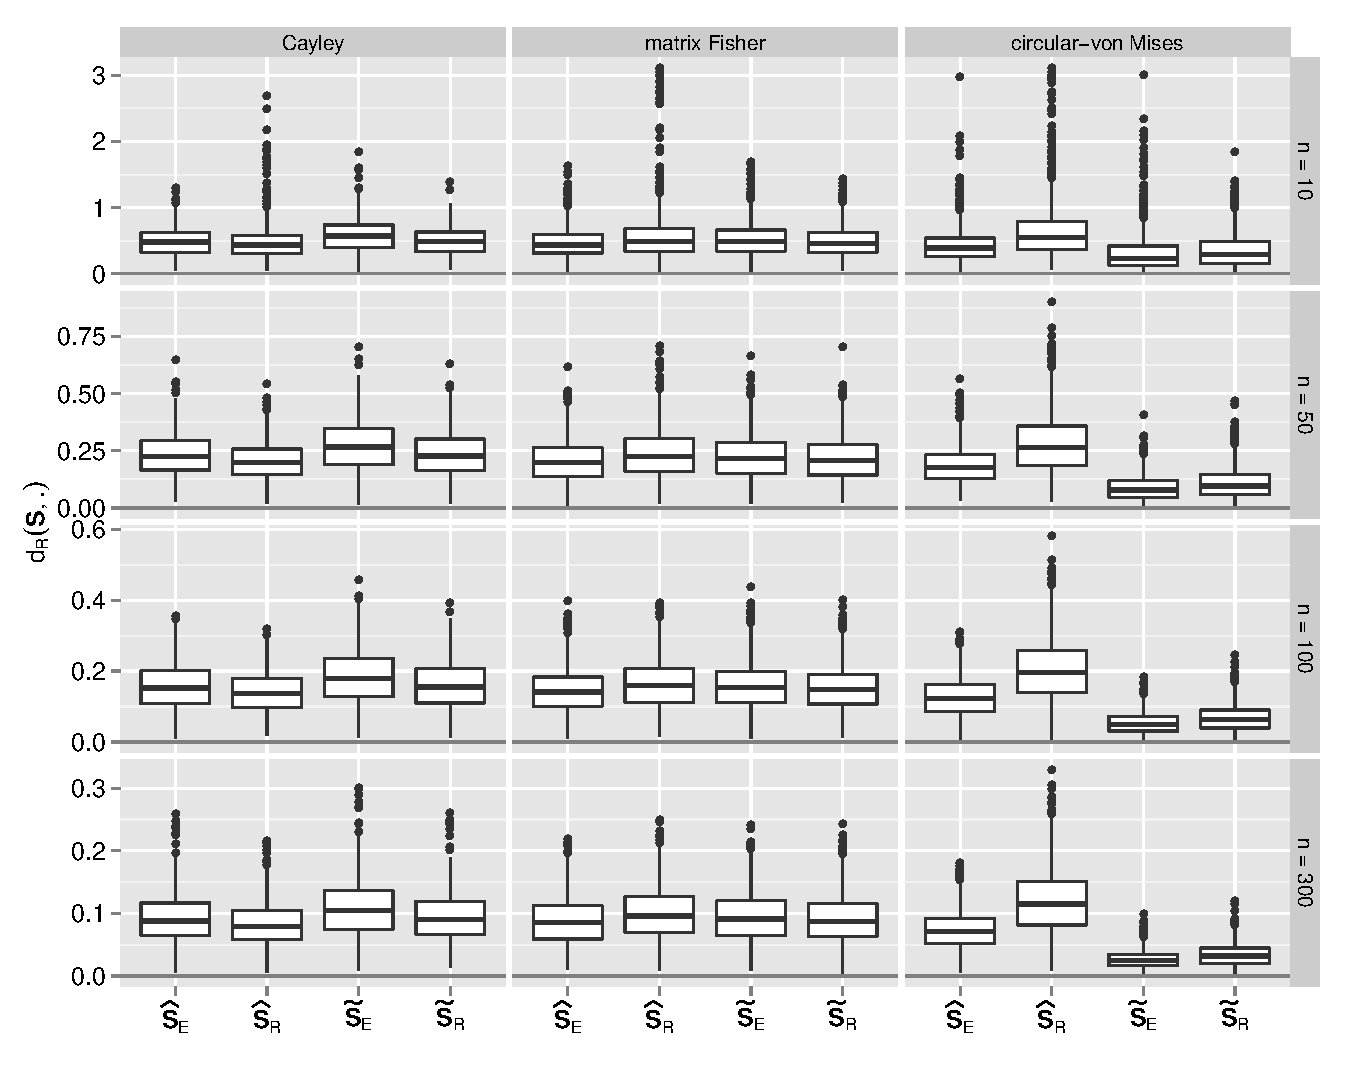
\includegraphics[width=1\textwidth]{Nu75AllNBoxes.pdf}
\caption{Box-plots of the estimation error for each rotation distribution and level of $n$,  $\nu=0.75$.}
\label{fig:NBoxes}
\end{figure}


%\begin{center}
%\begin{table}[h!]
%\caption{Numerical summaries of the estimation error  by distribution, $n=100$,  $\nu=0.25$.  The mean error (standard deviation) and RMSE are reported here.  \label{tab:alldN100Nu25}}
%\begin{tabular}{cccccccccc}
%  \hline
%		 &\multicolumn{3}{c}{\textbf{Cayley}} & \multicolumn{3}{c}{\textbf{matrix Fisher}}  & \multicolumn{3}{c}{\textbf{circular-von Mises}}\\ 
%Estimator &   Mean error  & RMSE& &  Mean error & RMSE& &   Mean error& RMSE \\  \hline \hline %\rule[2mm]{0mm}{3mm} 
% 		  $\GeomMean$  &  0.069 (0.0009)& 0.075 & &  0.070 (0.0009)& 0.076&  & 0.074 (0.0010)& 0.081 \\ 
% 		 $\ProjMean$ &   0.070 (0.0009)& 0.076 & &  0.070 (0.0009)& 0.076&  &  0.062 (0.0008)& 0.067\\ 
%		 $\GeomMedian$   & 0.077 (0.0010)& 0.083 & &  0.075 (0.0010)& 0.081&  & 0.027 (0.0005)& 0.031\\ 
% 		  $\ProjMedian$ & 0.079 (0.0010)& 0.086 & &  0.077 (0.0010)& 0.083 & & 0.026 (0.0005)& 0.030\\ \hline
%\end{tabular}
%\end{table}
%\end{center}

%\begin{center}
%\begin{table}[h!]
%\caption{Numerical summaries of the estimation error for all levels of $n$ for the circular-von Mises-based distribution,  $\nu=0.75$.}  \label{tab:vmnu75}
%\begin{tabular}{rccccrccc}
%  \hline
% $\mathbf{n}$ & \textbf{Estimator}  & \textbf{Mean error} & \textbf{RMSE} & &$\mathbf{n}$ & \textbf{Estimator} & \textbf{Mean error} & \textbf{RMSE} \\ \hline \hline
%   \multirow{4}{*}{10} & $\GeomMean$  & 0.652 & 0.789 &  & \multirow{4}{*}{100} & $\GeomMean$  & 0.204 & 0.222 \\ 
%    & $\ProjMean$  & 0.442 & 0.518 &   & & $\ProjMean$ & 0.128 & 0.139 \\ 
%    & $\GeomMedian$  & 0.366 & 0.459 &  &  & $\GeomMedian$  & 0.069 & 0.079 \\ 
%    & $\ProjMedian$  & 0.326 & 0.450 &   & & $\ProjMedian$  & 0.055 & 0.063 \\  
%    & & & & & & & \\ 
%    \multirow{4}{*}{50} & $\GeomMean$  & 0.280 & 0.309 &  &  \multirow{4}{*}{300} & $\GeomMean$  & 0.119 & 0.130 \\ 
%    & $\ProjMean$  & 0.185 & 0.202 &  &  & $\ProjMean$  & 0.075 & 0.081 \\ 
%    & $\GeomMedian$  & 0.109 & 0.130 &  & & $\GeomMedian$  & 0.034 & 0.039 \\
%    & $\ProjMedian$ & 0.088 & 0.105 &  &  & $\ProjMedian$ & 0.027 & 0.031 \\ 
%   \hline
%\end{tabular}
%\end{table}
%\end{center}

Finally, Figure 7 indicated how the choice of geometry affected the estimation error for both types of loss functions.  Tables \ref{tab:percL1} and \ref{tab:percL2} support these figures with an exact count (expressed as a percentage) of how often $\Rdist$ resulted in a smaller estimation error than $\Edist$.  Additionally, we give the average amount by which the $\Rdist-$ and $\Edist-$based estimates deviate from one another (along with a standard error estimate).  We denote the latter quantity by $\bar\delta$ where  $\delta=\Rdist(\ProjMedian,\bm S)-\Rdist(\GeomMedian,\bm S)$.   

\begin{table}[h]
\caption{Average reduction in estimation error by using $\GeomMedian$ instead of $\ProjMedian$, $\delta=\Rdist(\ProjMedian,\bm S) - \Rdist(\GeomMedian,\bm S)$ with standard error and percentage of samples for which $\Rdist(\GeomMedian,\bm S) < \Rdist(\ProjMedian,\bm S)$.}
\label{tab:percL1}
\centering
\scalebox{0.92}{
\begin{tabular}{crccccccccc}
  \hline
  %&&&\multicolumn{3}{c}{} & &\multicolumn{3}{c}{\textbf{matrix} } &&\multicolumn{3}{c}{\textbf{circular-}}\\
    &&&\multicolumn{2}{c}{\textbf{Cayley}} & &\multicolumn{2}{c}{\textbf{matrix Fisher}} & &\multicolumn{2}{c}{\textbf{circular-von Mises}}\\ 
\rule[2mm]{0mm}{3mm} 
  $\nu$&  $n$ && $\bar{\delta}$ (SE) & \% & & $\bar{\delta}$ (SE) & \% & & $\bar{\delta}$ (SE) & \% \\ 
  \hline \hline
\multirow{4}{*}{0.25}  
 &    10 && 0.0078 (0.0004) & 0.7430 && 0.0060 (0.0004) & 0.7250 && -0.0053 (0.0006) & 0.3280 \\ 
 &    50 && 0.0031 (0.0001) & 0.7830 && 0.0024 (0.0001) & 0.6970 && -0.0018 (0.0001) & 0.3270 \\ 
 &   100 && 0.0022 (0.0001) & 0.7890 && 0.0018 (0.0001) & 0.7120 && -0.0013 (0.0001) & 0.3080 \\ 
 &   300 && 0.0012 (0.0001) & 0.7810 && 0.0010 (0.0001) & 0.7110 && -0.0008 (0.0001) & 0.2840 \\
\hline
\multirow{4}{*}{0.50}   
  &    10 && 0.0315 (0.0016) & 0.7720 && 0.0171 (0.0017) & 0.6620 && -0.0192 (0.0020) & 0.3350 \\ 
  &    50 && 0.0126 (0.0005) & 0.8110 && 0.0055 (0.0006) & 0.6200 && -0.0081 (0.0005) & 0.2820 \\ 
  &   100 && 0.0085 (0.0003) & 0.8090 && 0.0047 (0.0004) & 0.6600 && -0.0047 (0.0003) & 0.3020 \\ 
  &   300 && 0.0049 (0.0002) & 0.8040 && 0.0024 (0.0002) & 0.6580 && -0.0027 (0.0001) & 0.2550 \\ 
\hline
\multirow{4}{*}{0.75}   
  &    10 && 0.0895 (0.0042) & 0.8210 && 0.0340 (0.0040) & 0.6330 && -0.0396 (0.0062) & 0.3220 \\ 
  &    50 && 0.0366 (0.0011) & 0.8660 && 0.0093 (0.0013) & 0.5970 && -0.0213 (0.0011) & 0.2380 \\ 
  &   100 && 0.0250 (0.0008) & 0.8580 && 0.0069 (0.0009) & 0.6030 && -0.0140 (0.0007) & 0.2400 \\ 
  &   300 && 0.0140 (0.0004) & 0.8500 && 0.0033 (0.0005) & 0.5890 && -0.0072 (0.0003) & 0.2180 \\   \hline
\end{tabular}}
\end{table}

\begin{table}[h!]
\caption{Average reduction in estimation error by using $\GeomMean$ instead of $\ProjMean$, $\delta=\Rdist(\ProjMean,\bm S) - \Rdist(\GeomMean,\bm S)$ with standard error and percentage of samples for which $\Rdist(\GeomMean,\bm S) < \Rdist(\ProjMean,\bm S)$.}  \label{tab:percL2}
\centering
\scalebox{0.92}{
\begin{tabular}{crcccccccccccc}
  \hline
  %& &&\multicolumn{3}{c}{} & &\multicolumn{3}{c}{\textbf{matrix} } &&\multicolumn{3}{c}{\textbf{circular-}}\\
    &&&\multicolumn{2}{c}{\textbf{Cayley}} & &\multicolumn{2}{c}{\textbf{matrix Fisher}} & &\multicolumn{2}{c}{\textbf{circular-von Mises}}\\ 
\rule[2mm]{0mm}{3mm} 
  $\nu$&  $n$ && $\bar{\delta}$ (SE) & \% & & $\bar{\delta}$ (SE) & \% & & $\bar{\delta}$ (SE) & \% \\  
  \hline \hline
\multirow{4}{*}{0.25} 
 &    10 && 0.0011 (0.0004) & 0.5210 && -0.0016 (0.0005) & 0.4500 && -0.0344 (0.0030) & 0.1280 \\ 
 &    50 && 0.0007 (0.0002) & 0.5310 && -0.0011 (0.0003) & 0.4350 && -0.0156 (0.0007) & 0.2090 \\ 
 &   100 && 0.0007 (0.0001) & 0.5650 && -0.0004 (0.0002) & 0.4690 && -0.0126 (0.0005) & 0.2010 \\ 
 &   300 && 0.0005 (0.0001) & 0.5880 && -0.0003 (0.0001) & 0.4860 && -0.0070 (0.0003) & 0.2390 \\\hline
\multirow{4}{*}{0.50}  
 &    10 && 0.0099 (0.0013) & 0.5920 && -0.0178 (0.0027) & 0.4340 && -0.1011 (0.0051) & 0.1570 \\ 
  &    50 && 0.0069 (0.0006) & 0.6450 && -0.0107 (0.0011) & 0.3920 && -0.0545 (0.0018) & 0.1450 \\ 
  &   100 && 0.0043 (0.0004) & 0.6420 && -0.0067 (0.0008) & 0.3930 && -0.0385 (0.0013) & 0.1620 \\ 
  &   300 && 0.0025 (0.0002) & 0.6420 && -0.0040 (0.0004) & 0.3930 && -0.0234 (0.0007) & 0.1570 \\ \hline
\multirow{4}{*}{0.75}  
  &    10 && 0.0163 (0.0062) & 0.6680 && -0.0958 (0.0105) & 0.3570 && -0.2101 (0.0113) & 0.1710 \\ 
  &    50 && 0.0257 (0.0012) & 0.7410 && -0.0356 (0.0045) & 0.3380 && -0.0955 (0.0032) & 0.1500 \\ 
  &   100 && 0.0169 (0.0009) & 0.7350 && -0.0240 (0.0043) & 0.3460 && -0.0763 (0.0021) & 0.1110 \\ 
  &   300 && 0.0091 (0.0005) & 0.7280 && -0.0124 (0.0009) & 0.3440 && -0.0446 (0.0012) & 0.1270 \\
   \hline
\end{tabular}}
\end{table}



%\begin{table}[h!]
%\caption{Results from an analysis of variance on the log transformed error data for $n=100$ and $\nu=0.25$ and treating distributions as blocks.  From this we can conclude that there is a statistically significant difference between the estimators.}
%\begin{center}
%\begin{tabular}{lrrrrr}
%  \hline
% & Df & Sum Sq & Mean Sq & F value & Pr($>$F) \\ 
%  \hline
%Distribution       & 2 & 927.61 & 463.80 & 1371.56 & $<1\times 10^{-5}$ \\ 
%Estimator   & 3 & 228.43 & 76.14 & 225.17 & $<1\times 10^{-5}$ \\ 
%Residuals   & 11994 & 4055.85 & 0.34 &  &  \\ \hline
%Total & 11999 & 5211.88 &&&\\
%   \hline
%\end{tabular}
%\end{center}
%\end{table}


\section{Sphere plots}
\label{sec:appendix.eyeballs}
Figures \ref{fig:eye-cayley} to \ref{fig:eye-vmises} show sphere plots for 100 samples from each of the Cayley, matrix Fisher and circular-von Mises distribution. The concentration parameter $\kappa$ in each distribution is chosen such that the samples have a circular variance of $\nu = 0.25$. The concentration of rotation matrices under circular-von Mises sampling is much higher to the origin (center of the circles) than for the two other distributions.


\begin{figure}
\centering
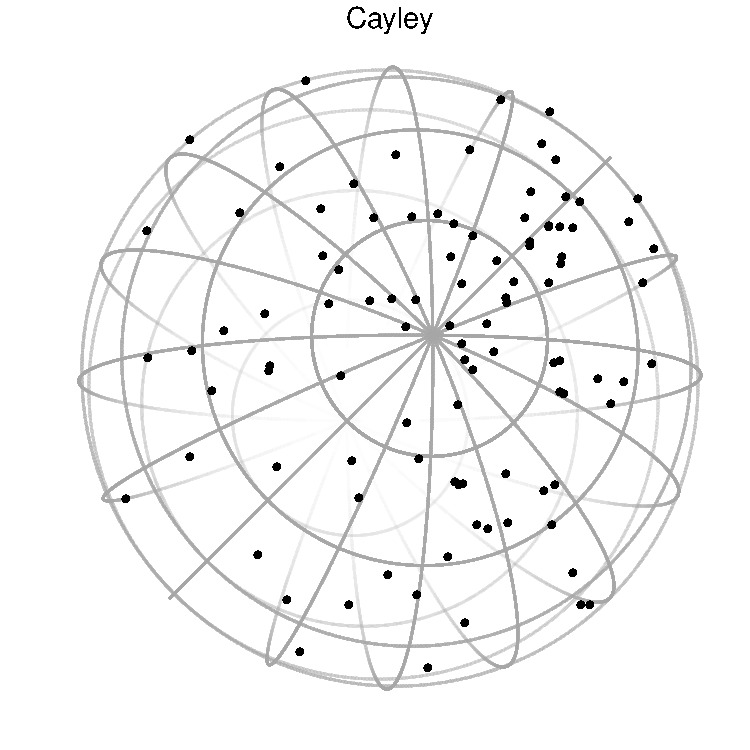
\includegraphics[width=.3\linewidth]{eye-cayley}
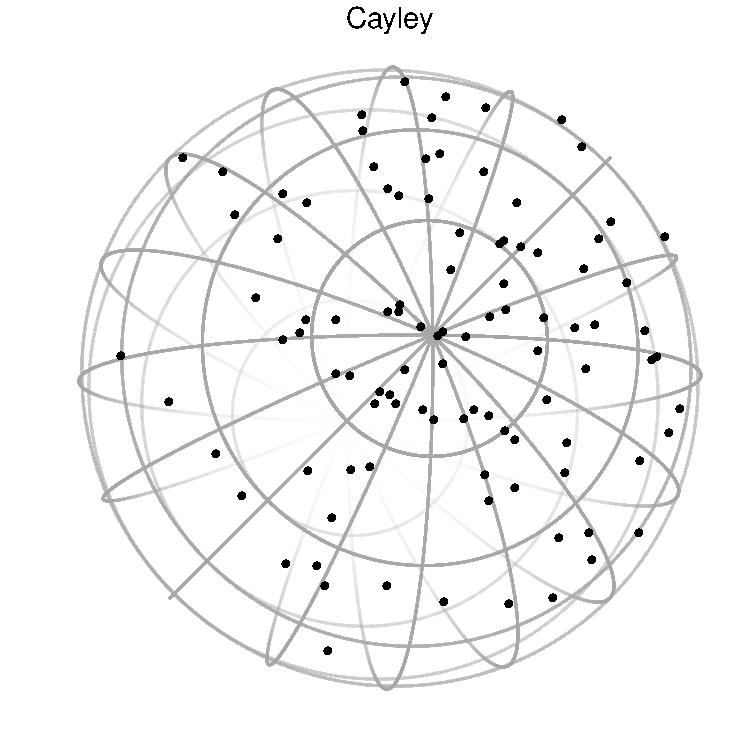
\includegraphics[width=.3\linewidth]{eye-cayley-2}
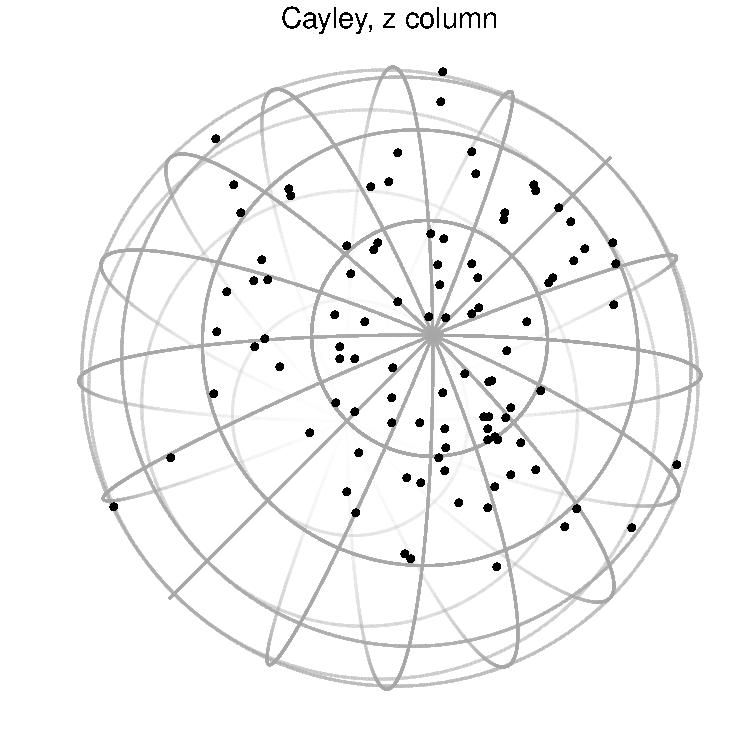
\includegraphics[width=.3\linewidth]{eye-cayley-3}
\caption{\label{fig:eye-cayley}Sphere plots for a sample of 100 rotations from a Cayley distribution with circular variance $\nu=0.25$}
\end{figure}
\begin{figure}
\centering
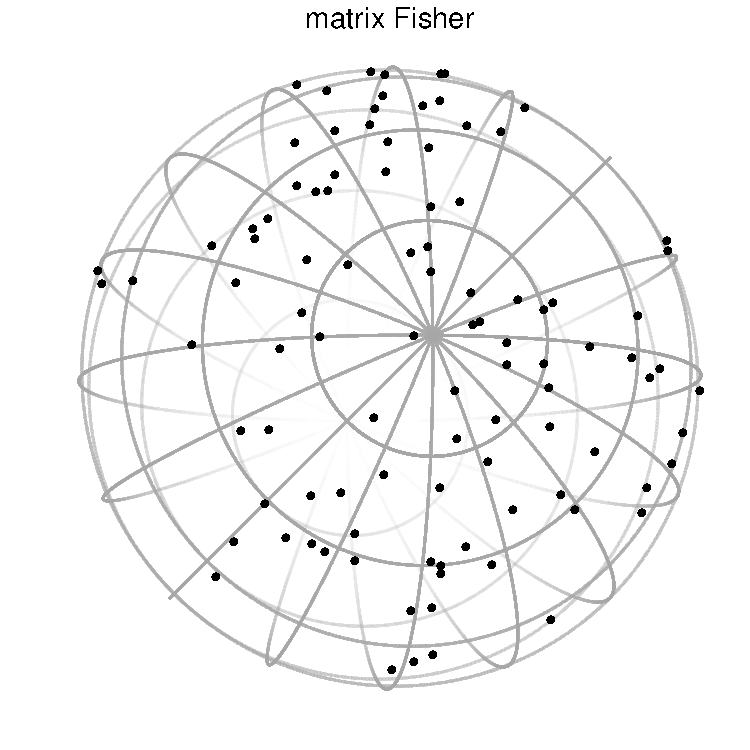
\includegraphics[width=.3\linewidth]{eye-fisher}
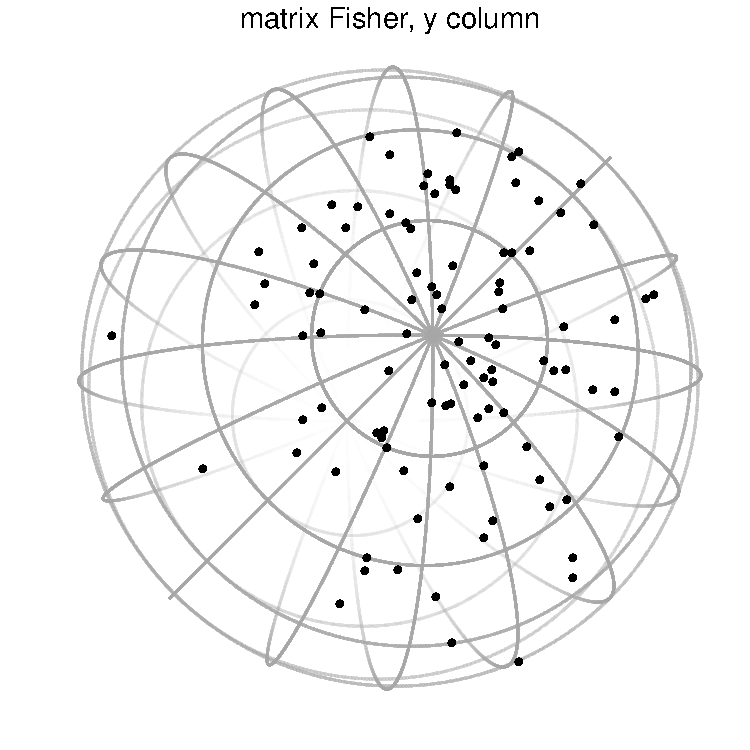
\includegraphics[width=.3\linewidth]{eye-fisher-2}
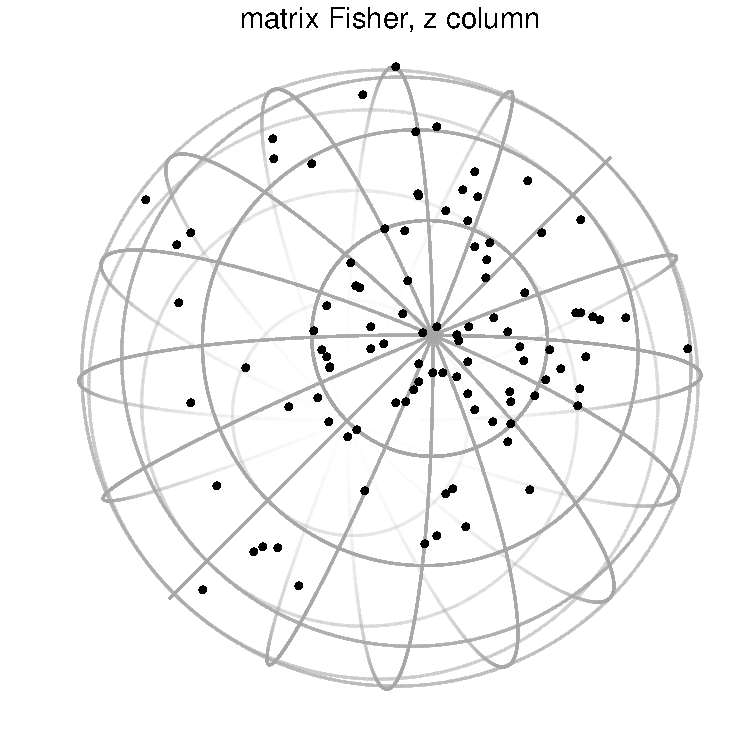
\includegraphics[width=.3\linewidth]{eye-fisher-3}
\caption{\label{fig:eye-fisher}Sphere plots for a sample of 100 rotations from a matrix Fisher distribution with circular variance $\nu=0.25$}
\end{figure}
\begin{figure}
\centering
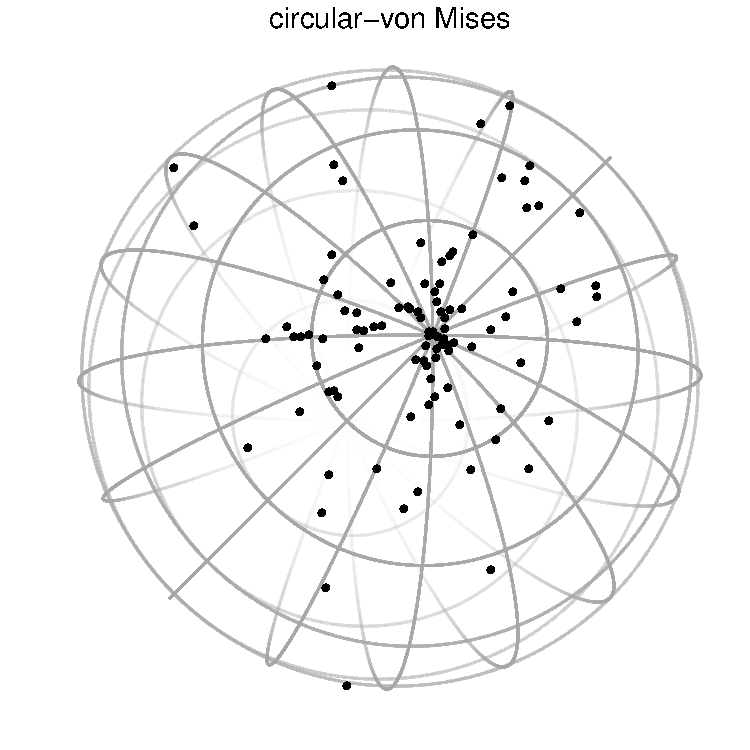
\includegraphics[width=.3\linewidth]{eye-vmises}
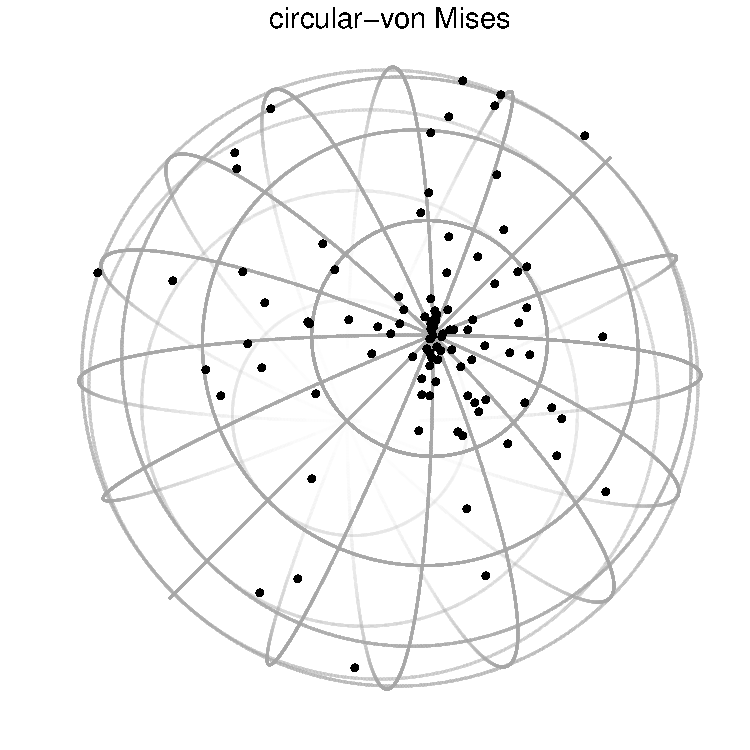
\includegraphics[width=.3\linewidth]{eye-vmises-2}
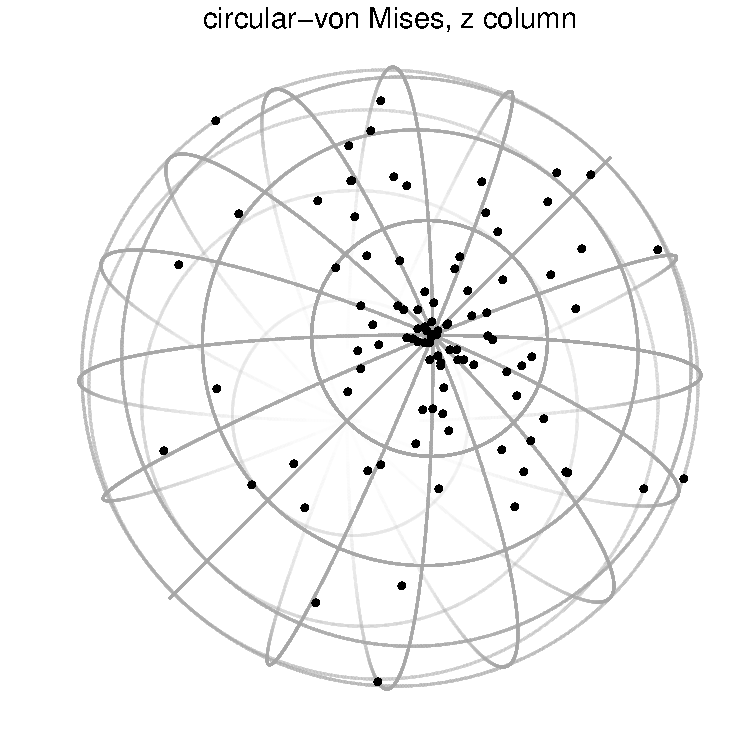
\includegraphics[width=.3\linewidth]{eye-vmises-3}
\caption{\label{fig:eye-vmises}Sphere plots for a sample of 100 rotations from a circular-von Mises distribution with circular variance $\nu=0.25$}
\end{figure}
\end{document}